\documentclass[../../Axiomathic.tex]{subfiles}

\begin{document}
\graphicspath{{sections/style/images/}{images/}}


\chapter{Theorem Style Guide}

This page is a visual test fixture for the Axiomathic website. It deliberately
contains each theorem-like environment from the shared preamble so that the web
palette can be reviewed in one place. It can be removed from the published
navigation later without changing the theorem definitions themselves.

\section{Core environments}

\begin{theorem}[Sample theorem]
If $a=b$ and $b=c$, then $a=c$.
\end{theorem}

\begin{lemma}[Sample lemma]
For every $n\in\N$, one has $n+0=n$.
\end{lemma}

\begin{prop}[Sample proposition]
The sum of two even integers is even.
\end{prop}

\begin{corollary}[Sample corollary]
Every integer divisible by $4$ is even.
\end{corollary}

\begin{defn}[Sample definition]
A positive integer $p>1$ is prime if its only positive divisors are $1$ and $p$.
\end{defn}

\begin{nota}[Sample notation]
We write $\eps>0$ for a small positive quantity and $\Z$ for the integers.
\end{nota}

\begin{conj}[Sample conjecture]
There are infinitely many primes of the form $n^2+1$.
\end{conj}

\begin{example}
The permutation $\cycle{1,2,3}$ is a $3$-cycle.
\end{example}

\begin{remark}
Remarks are deliberately quieter than the principal mathematical statements.
\end{remark}

\begin{warning}[Sample caution]
This is a visual warning/caution environment rather than a mathematical claim.
\end{warning}

\section{Notation rendering check}

The following line is included specifically to check custom MathJax macros:
\[
  \cycle{1,2,3,4}, \qquad \eps>0, \qquad \Z,\N,\Q, \qquad \lcm(6,8)=24.
\]


\section{Figure rendering checks}

These figures are included as a web-rendering test for image-rich pages. They
are not part of the mathematical style guide itself, but they let us check how
ordinary LaTeX figures, paired images and image grids are presented online.

\begin{figure}[htbp]
    \centering
    \begin{minipage}{0.46\textwidth}
        \centering
        
\includegraphics[width=0.86\linewidth]{00-01-06-0117-0001-Front.jpg}
        \par\small Front
    \end{minipage}\hfill
    \begin{minipage}{0.46\textwidth}
        \centering
        
\includegraphics[width=0.86\linewidth]{00-01-06-0117-0001-Rear.jpg}
        \par\small Rear
    \end{minipage}
    \caption{A side-by-side card deck image test.}
    \label{fig:style-side-by-side-deck}
\end{figure}

\begin{figure}[htbp]
    \centering
    \begin{tabular}{cccc}
        
\includegraphics[width=0.21\textwidth]{00-01-06-0117-0001-Front.jpg} &
        
\includegraphics[width=0.21\textwidth]{00-01-06-0117-0001-Rear.jpg} &
        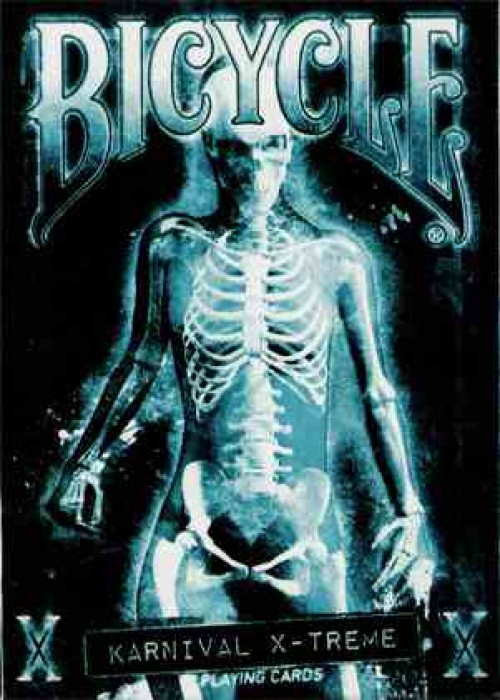
\includegraphics[width=0.21\textwidth]{00-01-06-0131-0001-Front.jpg} &
        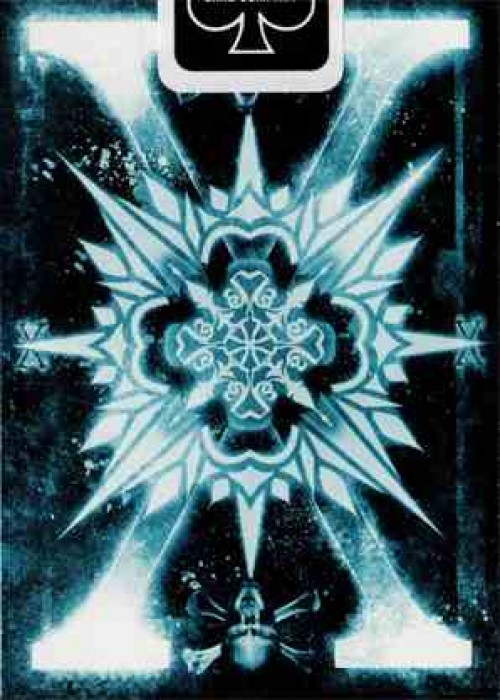
\includegraphics[width=0.21\textwidth]{00-01-06-0131-0001-Rear.jpg} \\
        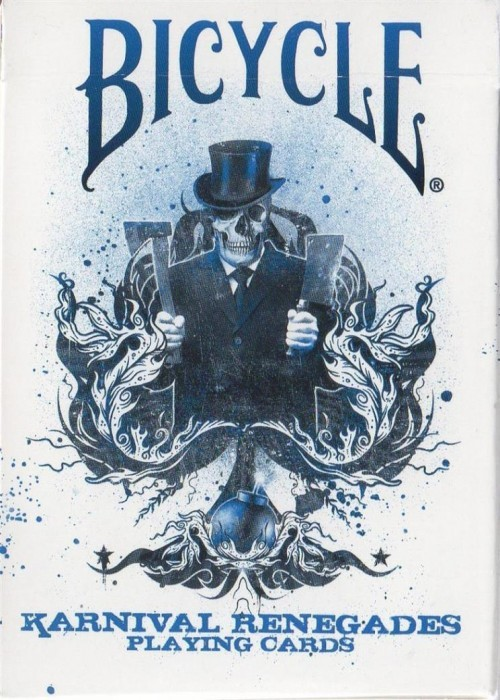
\includegraphics[width=0.21\textwidth]{XX-XXXX-XXXX-XX-Front.jpg} &
        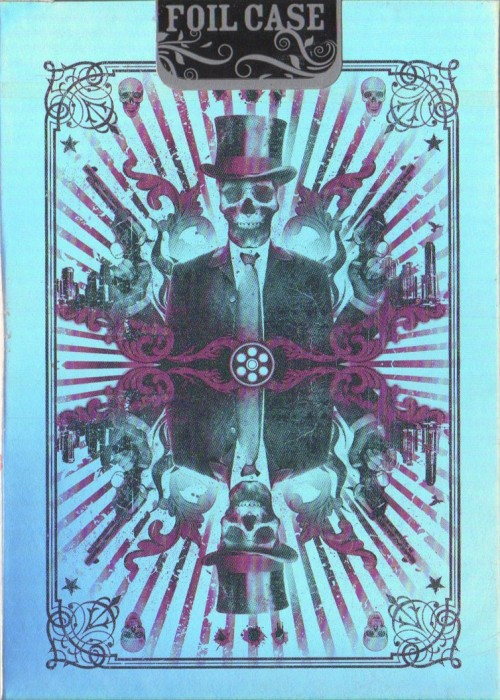
\includegraphics[width=0.21\textwidth]{XX-XXXX-XXXX-XX-Rear.jpg} &
        
\includegraphics[width=0.21\textwidth]{XX-XX-XX-XXXX-XXXX.jpg} &
        
\includegraphics[width=0.21\textwidth]{00-01-06-0117-0001-Front.jpg}
    \end{tabular}
    \caption{A $4\times 2$ image-grid rendering test.}
    \label{fig:style-four-by-two-grid}
\end{figure}

\end{document}
